\documentclass[usenames,dvipsnames,aspectratio=169]{beamer}

\usepackage[utf8]{inputenc}
\usepackage[T1]{fontenc}
\usepackage[magyar]{babel}
\usepackage{indentfirst}
\usepackage{listingsutf8}
\lstset{literate=
  {á}{{\'a}}1 {é}{{\'e}}1 {í}{{\'i}}1 {ó}{{\'o}}1 {ú}{{\'u}}1
  {Á}{{\'A}}1 {É}{{\'E}}1 {Í}{{\'I}}1 {Ó}{{\'O}}1 {Ú}{{\'U}}1
  {à}{{\`a}}1 {è}{{\`e}}1 {ì}{{\`i}}1 {ò}{{\`o}}1 {ù}{{\`u}}1
  {À}{{\`A}}1 {È}{{\'E}}1 {Ì}{{\`I}}1 {Ò}{{\`O}}1 {Ù}{{\`U}}1
  {ä}{{\"a}}1 {ë}{{\"e}}1 {ï}{{\"i}}1 {ö}{{\"o}}1 {ü}{{\"u}}1
  {Ä}{{\"A}}1 {Ë}{{\"E}}1 {Ï}{{\"I}}1 {Ö}{{\"O}}1 {Ü}{{\"U}}1
  {â}{{\^a}}1 {ê}{{\^e}}1 {î}{{\^i}}1 {ô}{{\^o}}1 {û}{{\^u}}1
  {Â}{{\^A}}1 {Ê}{{\^E}}1 {Î}{{\^I}}1 {Ô}{{\^O}}1 {Û}{{\^U}}1
  {œ}{{\oe}}1 {Œ}{{\OE}}1 {æ}{{\ae}}1 {Æ}{{\AE}}1 {ß}{{\ss}}1
  {ç}{{\c c}}1 {Ç}{{\c C}}1 {ø}{{\o}}1 {å}{{\r a}}1 {Å}{{\r A}}1
  {€}{{\EUR}}1 {£}{{\pounds}}1 {ő}{{\H{o}}}1
}
\usepackage{hyperref}
\usepackage{attachfile}
\usepackage{multirow}
% Navigációs pöttyök hozzáadása subsection nélküli fejezetekhez
\usepackage{remreset}
\makeatletter
\@removefromreset{subsection}{section}
\makeatother
\setcounter{subsection}{1}
%%%%%
\attachfilesetup{color={1.0 0.6 0.0},author={HFM},description={Kattintson duplán a minta %
megtekintéséhez!},icon=Paperclip}
\definecolor{kiemelesszin}{rgb}{0.6,0.0,0.0}
\definecolor{kiemelesszinZ}{rgb}{0.0,0.6,0.0}
\definecolor{kiemelesszinN}{RGB}{196,127,0}
\definecolor{hivatkozasszin}{rgb}{0.0,0.0,0.75}
\newcommand{\kiemel}[1]{{\color{kiemelesszin}#1}}
\newcommand{\kiemelZ}[1]{{\color{kiemelesszinZ}#1}}
\newcommand{\kiemelN}[1]{{\color{kiemelesszinN}#1}}
\newcommand{\hiv}[1]{{\color{hivatkozasszin}#1}}
\frenchspacing
\usetheme[compress]{Berlin}

\title[Web technológiák - HTML]{Egyszerű HTML5 weboldalak készítése}
\subtitle{(GKxB\_INTM049)}
\author{Dr. Hatwágner F. Miklós}
\institute{Széchenyi István Egyetem, Győr}
\date{\hiv{\href{https://github.com/wajzy/GKxB\_INTM049.git}{https://github.com/wajzy/GKxB\_INTM049.git}}\\ \today}

\begin{document}

%1
\begin{frame}[plain]
  \titlepage
\end{frame}

\section{Jelölőnyelvek}

%2
\begin{frame}
  \begin{itemize}
    \item Cél: a nyers szöveg egyes részeit strukturálni, jelentésbeli többletet hozzáadni (pl. fejezetcím, bekezdés)
    \item Történeti előzmény: nyomdai előkészítés, kéziratok szerkesztése, gépi szedőrendszerek
    \item Példák jelölőnyelvekre: 
      \hiv{\href{http://man7.org/linux/man-pages/man7/roff.7.html}{roff}}, 
      \hiv{\href{https://www.latex-project.org/}{LaTeX}}, 
      \hiv{\href{https://en.wikipedia.org/wiki/Standard_Generalized_Markup_Language}{SGML}}
  \end{itemize}
\end{frame}

\subsection{roff}

%3
\begin{frame}
  \footnotesize
  \begin{description}[m]
    \item[RUNOFF] \hfill \\ nyers szövegből és parancsokból (.XX) álló fájlok $\to$ tördelt megjelenítés buta terminálokon (OS: Compatible Time Sharing System, CTSS, 1963)
    \item[runoff] \hfill \\ a RUNOFF bővített képességű portja \emph{IBM Selectric} terminálokhoz (OS: Multiplexed Information and Computing Service, multics, $\approx$'60-as évek vége)
    \item[roff] \hfill \\ a runoff továbbfejlesztése a Bell Telephone Labs-nál (1973) a PDP-11 géphez kapcsolt \emph{Graphic Systems CAT} (grafikus szedőegység) miatt. A roff család:
    \begin{description}[m]
      \item[troff] \hfill \\ typesetter roff a CAT-hez
      \item[nroff] \hfill \\ terminálokhoz és nyomtatókhoz
      \item[roff] \hfill \\ korlátozott képességű runoff utód, nem fejlesztették tovább
    \end{description}
    \item[groff] \hfill \\ GNU implementáció, máig fejlesztik $\to$ man oldalak
  \end{description}
\end{frame}

%4
\begin{frame}
  \begin{columns}[c]
    \column{0.5\textwidth}
      \tiny
      \begin{exampleblock}{\textattachfile{groff.1}{/usr/share/man/man1/groff.1.gz/groff.1}}
        \lstinputlisting[language=,breaklines=true,linerange={1-3},numbers=left,firstnumber=1]{groff.1}
        \lstinputlisting[language=,basicstyle=\ttfamily,breaklines=true,postbreak=\mbox{\textcolor{red}{$\hookrightarrow$}\space},linerange={75-85},numbers=left,firstnumber=75]{groff.1}
      \end{exampleblock}
    \column{0.5\textwidth}
      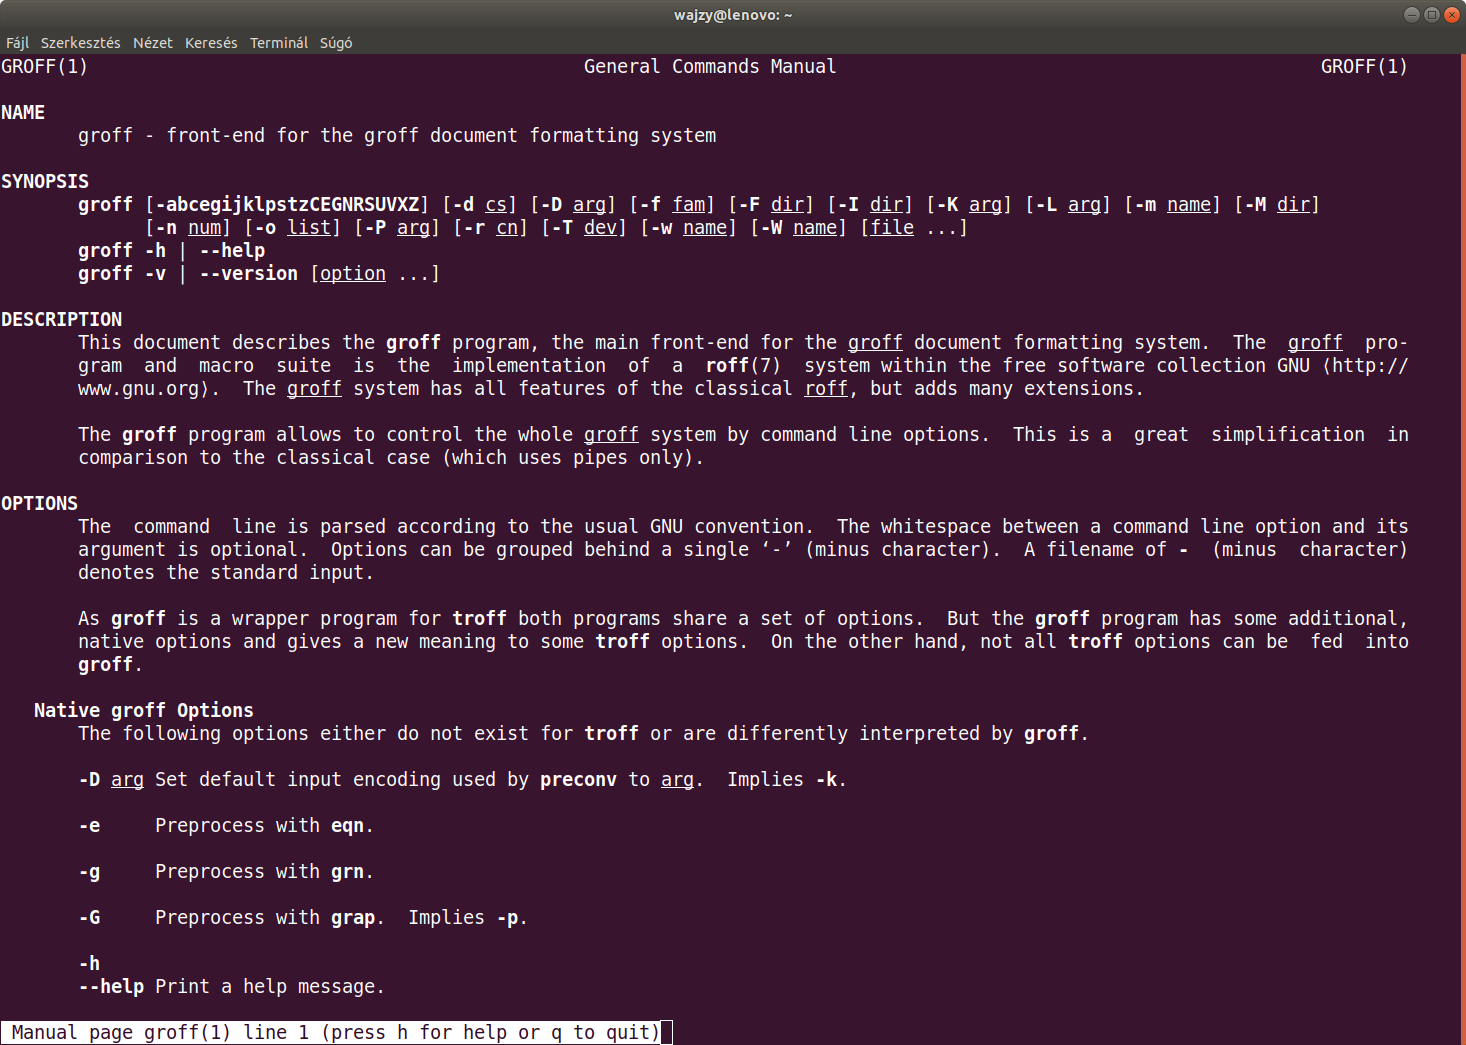
\includegraphics[width=\linewidth]{./groff.png}
  \end{columns}
\end{frame}

\subsection{\LaTeX{}}

%5
\begin{frame}
  \begin{columns}[T]
    \column{0.3\textwidth}
      \begin{description}[m]
        \item[\TeX] \hfill \\ Betűszedő rendszer, fejlesztője Donald E. Knuth, 1978 (Elégedetlenség \hiv{\href{https://www-cs-faculty.stanford.edu/~knuth/taocp.html}{könyvének}} szedésével.)
        \item[\LaTeX] \hfill \\ \TeX-en alapuló szövegformázó rendszer, Leslie Lamport, 1983
      \end{description}
    \column{0.7\textwidth}
        \begin{exampleblock}{\textattachfile{html.tex}{html.tex}}
          \centering
          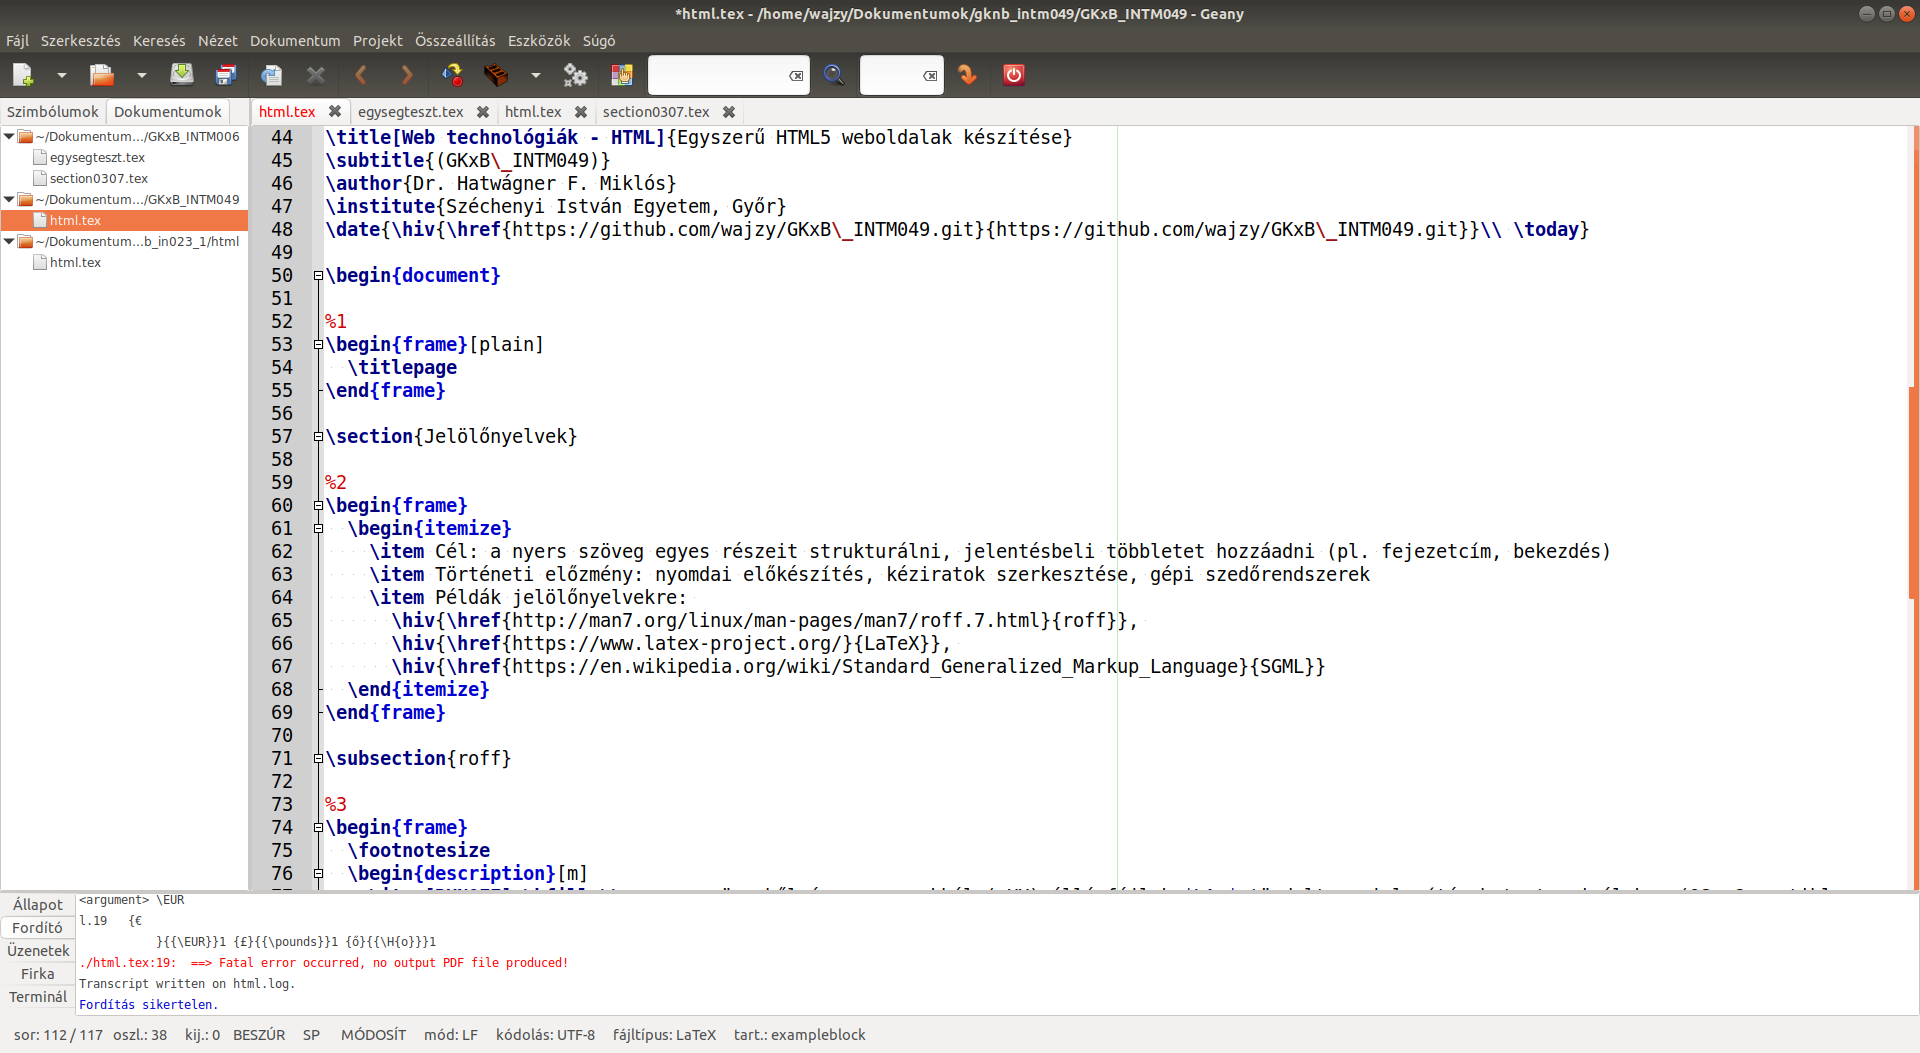
\includegraphics[scale=.14]{./latex.png}
        \end{exampleblock}
  \end{columns}
\end{frame}

\subsection{SGML}

%6
\begin{frame}
  \begin{itemize}
    \item SGML (Standard Generalized Markup Language), ISO 8879:1986
    \item Szabványos jelölőnyelv dokumentumok szerkezetének leírására,
beleértve a címkék definiálását is
    \item Gépfüggetlen metanyelv
    \item Előzménye: GML (1969)
    \begin{itemize}
      \item C. \kiemel{G}oldfarb (IBM), E. \kiemel{M}osher, R. \kiemel{L}orie
      \item dokumentumtípusonként egyedi kódolási séma definiálható
      \item előre definiált elemek egymásba ágyazhatóak
      \item először az IBM nyomdarendszere használta
    \end{itemize}
    \item Tulajdonságai
    \begin{itemize}
      \item Deklaratív: struktúrát és attribútumokat rögzít, nem a feldolgozás módját ($\to$~időtállóság)
      \item Gépi feldolgozás lehetősége
    \end{itemize}
  \end{itemize}
\end{frame}

%7
\begin{frame}
  \begin{itemize}
    \item Legfontosabb építőelemek
    \begin{itemize}
      \item Elemek ([element] nyitó és záró cimkék [tag] által határolva)
      \item A nyitó tagben attribútumok (kulcs-érték párok) adhatók meg
      \item Elemek egymásba ágyazhatóak
      \item Elemek, attribútumok alkalmazási szabályai $\to$ Document Type Definition (DTD)
    \end{itemize}
    \item Néhány korai, jelentős alkalmazás
    \begin{itemize}
      \item Electronic Manuscript Project of the Association of American Publishers (AAP, tudományos dokumentumok)
      \item Computer-aided Acquisition and Logistic Support (CALS, katonai dokumentumok kezelése)
      \item LinuxDoc (Linux csomagok)
    \end{itemize}
  \end{itemize}
\end{frame}

%8
\begin{frame}[fragile]
  \scriptsize
  \begin{columns}[T]
    \column{0.4\textwidth}
    \begin{exampleblock}{SGML példa}
      \begin{verbatim}
<!DOCTYPE PEOPLE SYSTEM 
  "people.dtd">
<PEOPLE DATE="15 6 2000">
 <NAME TITLE="Mr">
  <FIRST>Wally</FIRST>
  <LAST>Wallpaper</LAST>
 </NAME>
 <NAME>
  <LAST>Jackson</LAST>
 </NAME>
 <NAME TITLE="Dr">
  <FIRST>Susan</FIRST>
  <MIDDLE>Ramsay</MIDDLE>
  <LAST>Sukie</LAST>
 </NAME>
</PEOPLE>
\end{verbatim}
    \end{exampleblock}
    \column{0.6\textwidth}
    \begin{exampleblock}{people.dtd}
      \begin{verbatim}
<!ELEMENT people - - (name+)>
<!ATTLIST people date NUMBERS #REQUIRED>

<!ELEMENT name - - (first?, middle?, last)>
<!ATTLIST name title CDATA #IMPLIED>

<!ELEMENT first - - (#PCDATA)>
<!ELEMENT middle - - (#PCDATA)>
<!ELEMENT last - - (#PCDATA)>
\end{verbatim}
    \end{exampleblock}
    \tiny
    Forrás: \textattachfile{chap4.html}{OmniMark dokumentáció}
  \end{columns}
\end{frame}

\end{document}
